\chapter{System Development}
\label{ch:system-development}
This chapter will include the software specifications and the system's design with detailed information about our system including functional requirements, non-functional requirements, user requirements, system architecture, use case, data design following the logic in the \acrshort{srd} document.

\section{High Level Architecture}
Through results gathered from the previous chapter according analyzing and specifying the requirements of the project, we can now start the design step as it is a crucial and aim to undertake and prepare the ground for the implementation step. Figure \ref{fig:system-architecture} shows the overall high level architecture of the system.

\begin{figure}[!htb]
    \centering
    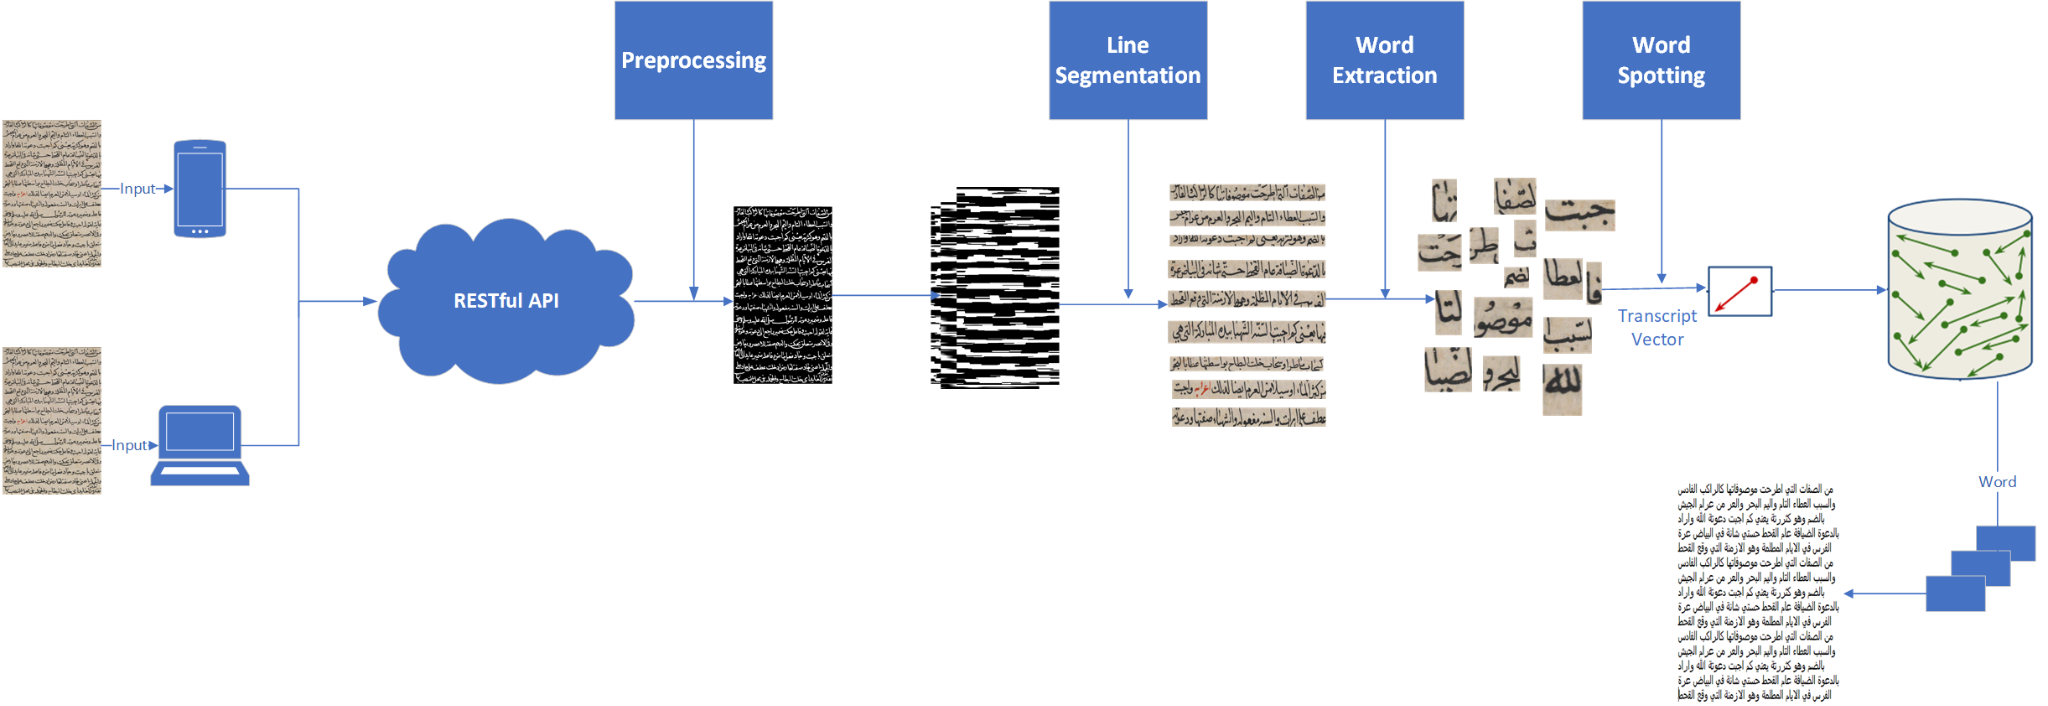
\includegraphics[width=17cm,height=8cm]{images/system-arch.png}
    \caption{High Level Project Architecture}
    \label{fig:system-architecture}
\end{figure}

\pagebreak

\section{Functional Requirements}
Defining correctly the requirements that our work is asked to satisfy, is one of the most important steps during our project development. During this chapter, we will analyze requirements within describing those that are functional and those that are non-functional. Then in a second section, we will define the structure and the dynamic behavior of the system, by introducing the interaction between its different actors and the entire system. \\

Functional requirements are directly related to system services. It help you capture files of the system’s intended behavior. This behavior can be expressed as functions, services, tasks, or any system required to perform. In this subsection, we list the functions that are required in our system.

\subsection{Business}
\begin{itemize}
  \item The system should be 85\% to 95\% accurate.
\end{itemize}

\subsection{Authentication}
\begin{itemize}
  \item The sign up of all users would be done by the admin panel. \\
        To sign up into the system, the basic information of the user would be required and will be added to the system.
  \item The system will allow the user to continue as a guest or anonymous account. \\
  The guest account will not require any sign up process and didn't keep track users history.
\end{itemize}

\subsection{Dashboard}
\begin{itemize}
 \item The admin panel would display the overall previous predictions that the user had made it.
 \item Admin panel would have different tabs that redirect to the prediction page or back to home page.
 \item The list of predictions shown in the admin panel, each one will have the image and buttons for downloading and deleting that prediction.
\end{itemize}

\subsection{Classification}
\begin{itemize}
 \item The user will be able to add/upload an image into the system to be predicted and return the results.
 \item On clicking predict, the system will show the results of the image on the screen.
 \item The system will allow the user to crop the uploaded image before predicting process, to enable the user control on which area need to apply on.
\end{itemize}

\section{Non functional Requirements}
Following are the non-functional requirements of our system
\begin{enumerate}
  \item \textbf{Security:} The user's data that would be required during sign up should be confidential, safe, and secure.
  \item \textbf{Performance:} The system should less than a minutes to process the image and displays the results.
  \item \textbf{Compatible:} The system should be compatible with all browsers and Android devices.
  \item \textbf{Memory Efficient:} The mobile application should be space efficient and should occupy large space of memory.
  \item \textbf{Usability:} The interface of the system should be simple and flow of app should be understandable by anyone that non-technical person.
  \item \textbf{Scalability:} The system should be scalable so that it can later be used in real world or at industry level.
  \item \textbf{Maintainability:} The system should be easily maintainable so that it can become more advance and efficient when use in industry.
  \item \textbf{Documentation:} The solution should be well-documented in order to provide the best use for the costumer.
\end{enumerate}

\pagebreak

\section{Use Cases}
The use case diagram captures the behaviour of a software system. This diagram describes the various actions, which can be made by an outside user. It splits the feature of the system into coherent units, the use cases, having a sense for the actors. This section presents detailed use cases of our system. The figure \ref{fig:use-case-digram} shows the general use case diagram that includes the common functionalities for all components. \\

\begin{figure}[H]
    \centering
    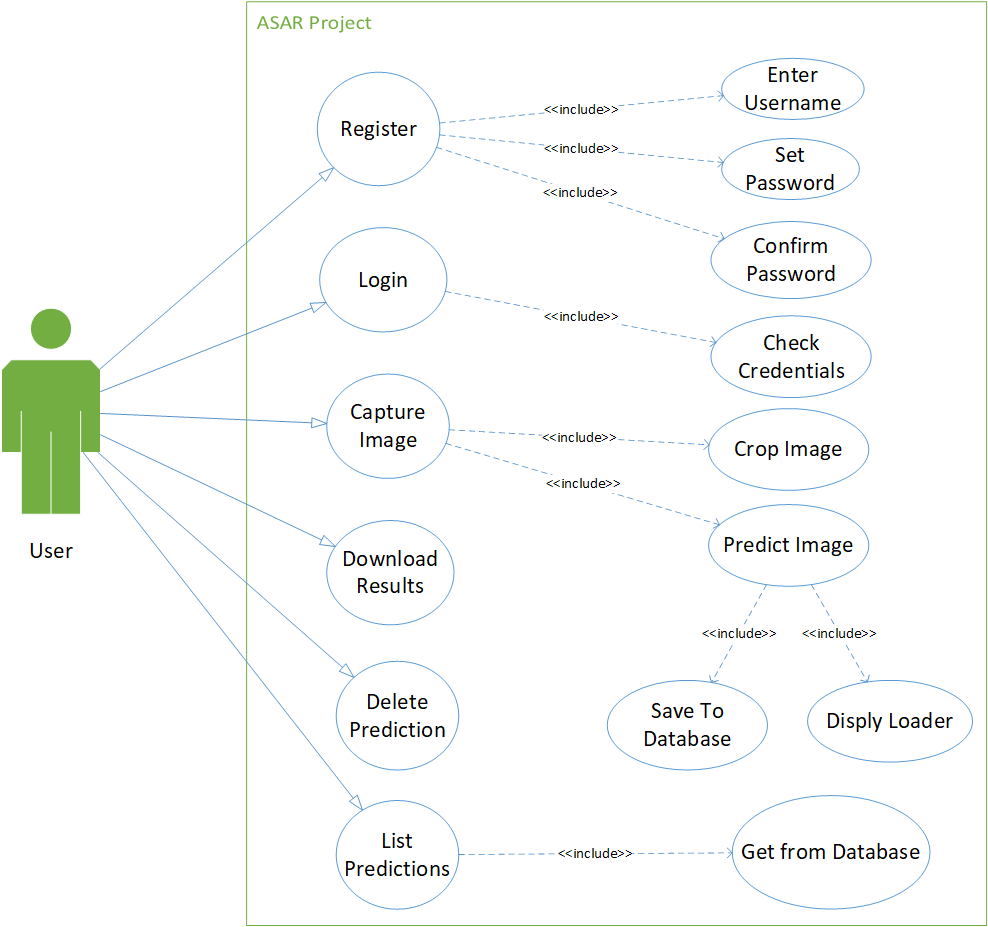
\includegraphics[width=14cm]{images/use case.png}
    \caption{Use Case Diagram}
    \label{fig:use-case-digram}
\end{figure}

\pagebreak
\noindent
In order to clarify the previous diagram, we present a detailed description of the most important use cases in the following tables. \\

\noindent
\textbf{Use Case 1: Login}
\begin{table}[H]
    \centering
    \begin{tabular}{|l|p{.60\textwidth}|p{0.30\textwidth}|}
    	\hline
    	Use-Case Name: & Login\\ \hline
    	Use-Case ID:& UC-01 \\\hline
    	Priority:& High\\ \hline
    	Source:& None \\ \hline
    	Primary Business Actor: & User \\ \hline
    	Other Participating Actors:&  No one\\ \hline
    	Description:&  The user would login the application as well as admin panel to use the system. Only authenticated users will be allowed to login. \\ \hline
    	Precondition:&  User must be registered. \\ \hline
    	Trigger:&  When user enters his credentials and clicks on submit. \\ \hline 
    	Typical course of events:&  \textbf{Actor Action:}
    	\begin{enumerate}
    		\item 	User enters the credentials and clicks on submit button.
    	\end{enumerate}
    
    	\vspace{2mm}
    	
    	\textbf{System Action: }
    	\begin{enumerate}
    		\item System checks the credentials of the user and validate them.
    		\item 	If the credentials are valid. User is allowed to use the system, else error generated. 
    	\end{enumerate}
    	\\ \hline
    	Conclusion:  & If credentials are valid, them user will logged in.\\ \hline
    	Post Condition: & None \\ \hline
    \end{tabular}\\
\end{table}

\pagebreak

\noindent
\textbf{Use Case 2: Capture Image}

\begin{table}[H]
    \centering
    \begin{tabular}{|l|p{.60\textwidth}|p{0.30\textwidth}|}
    	\hline
    	Use-Case Name: & Capture Image\\ \hline
    	Use-Case ID:& UC-02 \\\hline
    	Priority:& High\\ \hline
    	Source:& None \\ \hline
    	Primary Business Actor: & User \\ \hline
    	Other Participating Actors:&  No one\\ \hline
    	Description:&  The user would upload or capture the image of manuscript from the front and side view. The user can crop that image with desired area for classifying.  \\ \hline
    	Precondition:&  User must be authenticated. \\ \hline
    	Trigger:&  When user is logged in into the system and click on the upload/camera buttons to capture image. \\ \hline 
    	Typical course of events:&  \textbf{Actor Action:}
    	\begin{enumerate}
    		\item 	The user clicks on the button to upload/capture image.
    	\end{enumerate}
    
    	\vspace{2mm}
    	
    	\textbf{System Action: }
    	\begin{enumerate}
    		\item After capturing the image, the image is sent to server for further processing and predicting.
    	\end{enumerate}
    	\\ \hline
    	Conclusion:  & The image is captured by mobile and web applications with cropped ability to be sent to the server for further processing.\\ \hline
    	Post Condition: & The image is sent to the server for further processing. \\ \hline
    \end{tabular}\\
\end{table}

\pagebreak

\noindent
\textbf{Use Case 3: Predict Image}
\begin{table}[H]
    \centering
    \begin{tabular}{|l|p{.60\textwidth}|p{0.30\textwidth}|}
    	\hline
    	Use-Case Name: & Predict Image\\ \hline
    	Use-Case ID:& UC-03 \\\hline
    	Priority:& High\\ \hline
    	Source:& None \\ \hline
    	Primary Business Actor: & User \\ \hline
    	Other Participating Actors:&  No one\\ \hline
    	Description:&  When the user prepare image by uploading and cropping it, the recognizing transcripts of the image will be generated and stored in the system's database  \\ \hline
    	Precondition:&  User must be authenticated. \\ \hline
    	Trigger:&  When user clicks on the predict button. \\ \hline 
    	Typical course of events:&  \textbf{Actor Action:}
    	\begin{enumerate}
    		\item 	The user clicks on the button recognizing image content.
    	\end{enumerate}
    
    	\vspace{2mm}
    	
    	\textbf{System Action: }
    	\begin{enumerate}
    		\item The system take this image and predicting the content of it to generate corresponding transcripts.
    		\item The system take these transcripts as result and store it to the database and return it for user's screen.
    	\end{enumerate}
    	\\ \hline
    	Conclusion:  & The results is return to user's screen and new record is saved into the database \\ \hline
    	Post Condition: & The results can be shown through user's screen. \\ \hline
    \end{tabular}\\
\end{table}

\pagebreak

\section{Data Design}
This section presents the different diagrams for clarifying our system data design. We will represent in detail the \acrshort{uml} class diagram to present our database structure and relationships between entities. UML class diagram and gives a brief description of each class in our system. Attributes and methods of each class and relationship among classes are clearly presented. Our project contains the following classes shown in figure \ref{fig:class-digram}.

\begin{figure}[!htb]
    \centering
    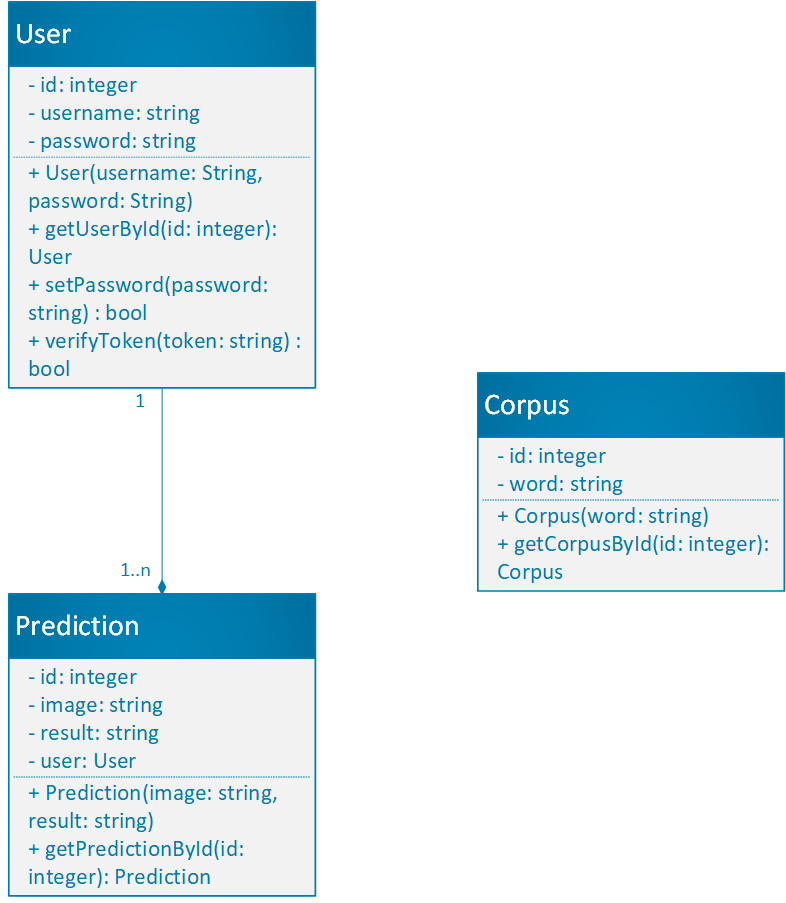
\includegraphics[width=10cm]{images/class diagram.png}
    \caption{Class Diagram}
    \label{fig:class-digram}
\end{figure}

\begin{itemize}[itemsep=1pt, topsep=5pt]
    \item   \textbf{User}: \\
    This class represents a generic user in our system. The class encapsulates information like username, password for a particular instance of a user.
    \item   \textbf{Prediction}: \\
    This class represents the prediction results that done by a user to be saved as a history for previous predictions. The class encapsulates information like image path that saved in the server, and the result for that image by particular user. 
    \item   \textbf{Corpus}: \\
    This class represents a collection of possible Arabic words to be used in recognizing process to generate the corresponding transcript.
\end{itemize}  

\pagebreak

\section{Architecture Design}
The software architecture is structured around main 4 layers. Every layer present a different psychical level of the application structure. Figure \ref{fig:architecture-diagram} shows the architecture diagram of our system.

\begin{figure}[!htb]
    \centering
    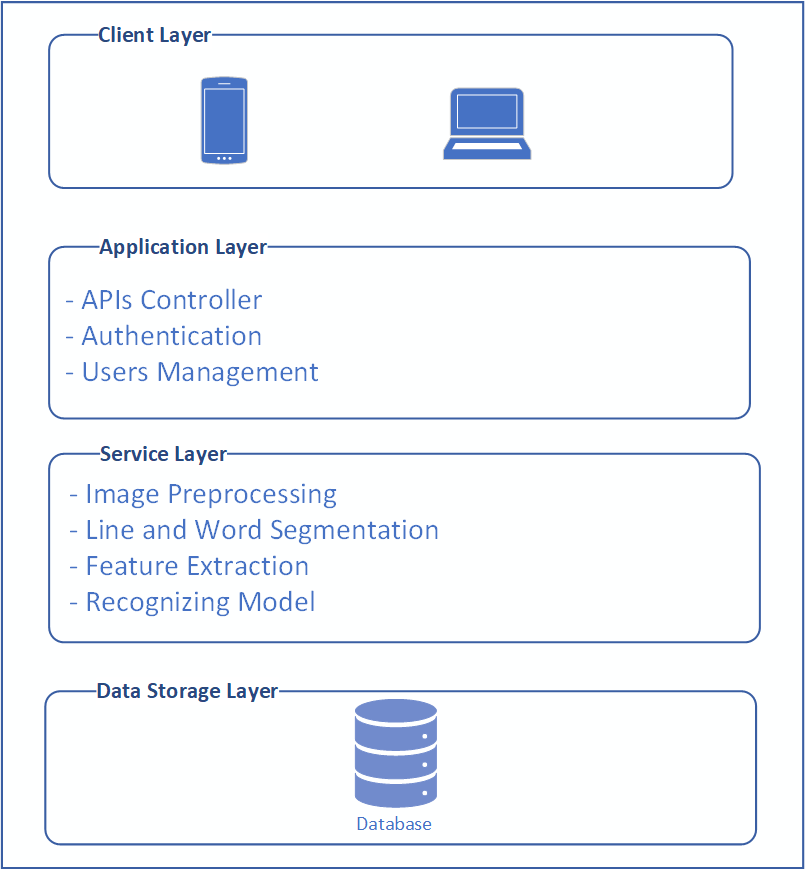
\includegraphics[width=10cm]{images/architecture layers.png}
    \caption{Architecture Diagram}
    \label{fig:architecture-diagram}
\end{figure}

\begin{itemize}[itemsep=1pt, topsep=5pt]
    \item   \textbf{Client Layer}: Is a display level of the application, includes the web view in the browser and the mobile view for the users.
    \item   \textbf{Application Layer}: Is the web server that executes and handles the different components of our application core. 
    \item   \textbf{Service Layer}: Is the application core for predicting the manuscript document image using the different steps like line, word segmentation and generate the corresponding transcripts.
    \item   \textbf{Data Storage Layer}: Is the layers where users' data, prediction histories are stored. 
\end{itemize}
